

\documentclass{article} 
\usepackage{todonotes}
\usepackage{graphicx}
\usepackage{grffile}
\usepackage{algorithm}
\usepackage[noend]{algpseudocode}
\usepackage{float}
\usepackage[font=footnotesize,labelfont=bf]{caption}
\usepackage[left=0.8in, right=0.8in, top=0.9in, bottom=1in]{geometry}
\usepackage{hyperref} 
%\usepackage{caption}
\graphicspath{ {images/} }


\title{ \textbf {\vspace{0.1cm}\Huge Parallel Jacobi\\ \vspace{0.3cm}}
 Final Project for the SPM course \vspace{0.5cm}\\} 

\date{\vspace{1.0cm}}

\author{ \Large Francesco Balzano \vspace{0.3cm}\\ 
%Matricola 541533 \vspace{0.5cm}\\
\Large Master Degree in Computer Science and Networking \vspace{0.4cm} \\
\Large A.Y. 2016-2017 
}


\begin{document}
  \pagenumbering{gobble}
  \maketitle
  %\newpage
  \noindent\rule{18cm}{0.4pt}
  \tableofcontents
  \newpage
  \pagenumbering{arabic}

\clearpage
\setcounter{page}{2}
  
\section{Problem}
Write a parallel application that finds the solution of a system of linear equations using the Jacobi iterative method. 
\section{Dependency analysis} \label{dep_an}
The algorithm iterates until either the maximum number of iterations is reached or a stopping condition occurs (\textit{e.g.} a convergence condition). \\
Basically, at each iteration the algorithm computes the following equations:
\[
\left\{ 
\begin{array}{c}
\sigma\textsubscript{i} = \displaystyle\sum_{j \neq i}^{} A_{i,j} \: X_{j}^{(k)}       \\
X_{i}^{(k+1)}  = \frac{1}{A_{i,i}} (b_{i} - \sigma\textsubscript{i})                    \\ 
\end{array}
\right. 
\]

$\forall i = 1, ... , n $. \\ \\

Unfortunately, the two equations cannot be parallelized because they violate the Bernstein conditions. Indeed, if we consider the same iteration of the algorithm, a \textit{READ-AFTER-WRITE} dependency holds for $\sigma\textsubscript{i}$. We cannot even parallelize the second equation at step \textit{K} and the first equation at step \textit{K+1}, because in that case it hods a \textit{READ-AFTER-WRITE} dependency on $X$. So the $X_{i}^{(k+1)}$ can be started to be computed only after $X_{i}^{(k+1)}$ has been computed. 

\begin{figure}[h]
\centering
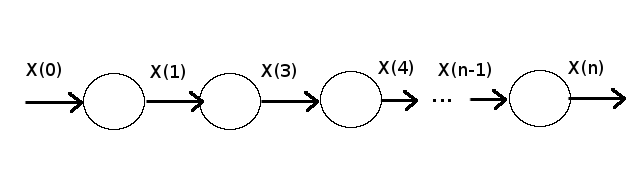
\includegraphics[scale=0.43]{dependency_chain}
\caption{Chain of dependencies}
\label{fig:dep_chain}
\end{figure}     

\section{Decomposition strategies}
I analyze some alternative strategies to turn the problem into a set of concurrent activities. Each alternatice is characterized by a different level of granularity for the concurrent activities. In the followingI am assuming that the concurrent activities are instantiated inside a loop of a single processing elements, so the time to setup them is fully paid. Instead, once setup they can go in parallel, and so when assessing the communication time I have considered the slowest of the communications that must be serialized.

\subsection{Tree of concurrent activities}
Each worker $W_{i,j}$ receives $A_{i,j}$ and $X_{j}$ and computes $A_{i,j} * X_{j}^{(k)}$ 
\paragraph{Performance model} In order to save some Workers, I map the computations onto the array $[W_{1,1}, ... ,W_{n,n}]$ . \\

\begin{figure}[h]
\centering
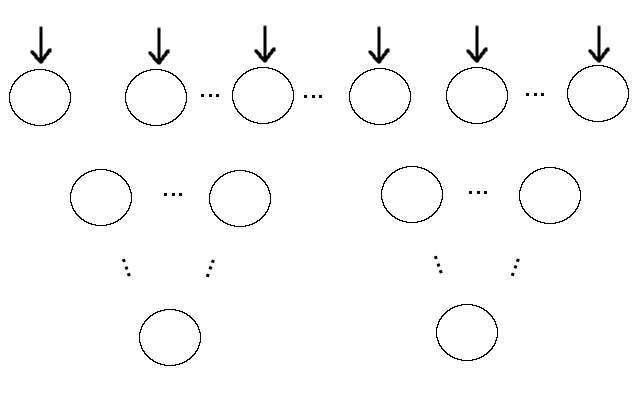
\includegraphics[scale=0.43]{tree_ca}
\caption{Decomposition strategy number 1: tree of workers}
\label{fig:tree_ca}
\end{figure} 

\begin{itemize}
\item \textbf{Number of Workers:} $n^2$
\item \textbf{Height(tree):} $O(\log n)$. Indeed the tree is made of n, independent subtrees, without cross edges between different subtrees.
\item Each level of the tree can be computed in parallel
\item \textbf{Calculation:} $T_{calc} = O(1) \: T_{aritm}$. Indeed the single Worker does a constant number of arithmetic operations.
\item \textbf{Overhead:} $O(n^2) \: T_{setup} + O( \log n) \: T_{comm}$. Indeed we have to setup $O(n^2)$ concurrent activities and the communications that are seriaized are proportional to the height of a tree with n leaves. The communication cost is given by the path in the subtree (from one leave to the root) that is slowest to be computed.
\end{itemize}


\subsection{Array of concurrent activities}
Each worker $W_{i}$ receives $A_{i,*}$ and $X^{k}$ and computes $X_{i}^{(k+1)}$, \textit{i.e.} it computes the system of section \ref{dep_an} for some $i \in {1,2, ... , n}$.
\paragraph{Performance model} 

\begin{figure}[h]
\centering
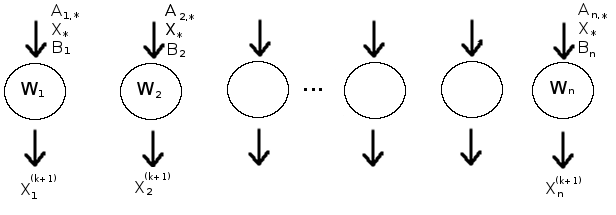
\includegraphics[scale=0.43]{array_ca}
\caption{Decomposition strategy number 2: array of workers}
\label{fig:array_ca}
\end{figure} 

\begin{itemize}
\item \textbf{Number of Workers:} $n$
\item \textbf{Calculation:} $T_{calc} = O(n) \: T_{aritm}$. Indeed the single Worker makes approximately $O(n)$ sums and $O(n)$ multiplications.
\item \textbf{Overhead:} $O(n) \: T_{setup} + O(1)  \: T_{comm}$. Indeed we have to setup $O(n)$ concurrent activities and the communications of the n Workers can go in parallel.
\end{itemize}

\subsection{Array of concurrent activities with pipeline}
Since the computation of the worker now takes a time linear and not constant we could try to lower the service time by inserting a 2-stage pipeline. In this new parallelization, the first stage of the pipeline that parallelizes $W_i$ computes $\sigma\textsubscript{i}$, while the second stage computes $X_{i}^{(k+1)}$. We are forced to build this exact configuration of the pipeline because we must keep into account the data dependencies already pointed out in section \ref{dep_an}.\\ 
\paragraph{Performance model} It is very likely that this parallelization is not worth it, because stage one takes $O(n) \: T_{aritm}$ while stage 2 takes $O(1) \: T_{aritm}$  . \\

\begin{figure}[h]
\centering
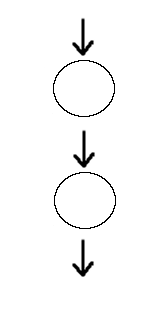
\includegraphics[scale=0.43]{single_worker_pipe}
\caption{Decomposition strategy number 2, variant with pipeline: only one worker is considered}
\label{fig:w_pipe}
\end{figure} 

\subsection{Single concurrent activitiy}
We consider a single worker $W$ that receives $A$ and $X$ and computes $X^{(k+1)}$, \textit{i.e.} it computes the system of section \ref{dep_an} $\forall i \in 1, ... , n $. .
\paragraph{Performance model} 

\begin{figure}[h]
\centering
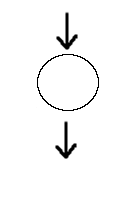
\includegraphics[scale=0.43]{single_worker_p3}
\caption{Decomposition strategy number 3: single worker}
\label{fig:worker}
\end{figure} 

\begin{itemize}
\item \textbf{Number of Workers:} $1$
\item \textbf{Calculation:} $T_{calc} = O(n^{2}) \: T_{aritm}$. 
\item \textbf{Overhead:} $O(1) \: T_{setup} + O(1)  \: T_{comm}$, if we instantiate the concurrent activity on a processing element different from the one running the main flow of control. If instead we instantiate the worker on the very same processing element, then the overhead is zero.
\end{itemize}

\section{Implementation} I decided to implement the second decomposition strategy, because is the one that according to me ffers the best tradeoff ``Parallelism Degree VS Overhead''. In this section I describe the main points concerning implementation decisions. While in the previous section I considered a single iteration of the Jacobi method, now I take into account that it is an iterative method. \\
The problem is a \textbf{data parallel} one: so I can consider a \textbf{map} decomposition. I must take into account the following features:
\begin{itemize}
\item \textbf{Split} of the data to be sent to the workers. This is tipically done by a \textbf{scatter} process, that sends the appropriate partition to each Worker, but since:
	\begin{itemize}
	\item $W_{i}$ reads only $A_{i,*}$ and $X^{k}$ 
	\item $W_{i}$ writes $X_{i}^{(k+1)}$, but it is the \textit{only one} that makes such write
	\item I target a \textit{shared-memory} architecture.
	\end{itemize}
I avoid using a scatter process that sends to each Worker the partition of data on which it has to do the computation. Instead, I will merge the scatter and the gatherer process into a single processing element and will assign the appropriate partitions to each worker only once at creation time.
\item \textbf{Computation} done by each Worker $W_{i}$: at initialization time each worker is simply provided a reference to $A, X$ and $B$ and the index $i$. After the computation, it updates $X_{i}^{(k+1)}$ in memory and tells the scatter that it has completed the current iteration.
\item \textbf{Gathering} of the results: the \textbf{gatherer} process waits that all the $W_{i}$ have concluded the computation for the current iteration and then:
	\begin{itemize}
	\item either stop the Workers and output the final $X$;
	\item or notify all the Workers to go on with another iteration.
	\end{itemize}
As already pointed out, I merge the scatter and the gatherer into a single process. This allows me to save one processing element and to have a centralized ``Locus of Control'' to control the execution of the program. \\
\end{itemize}
So the structure of the chosen parallelization is basically a map without the gatherer.

\begin{figure}[h]
\centering
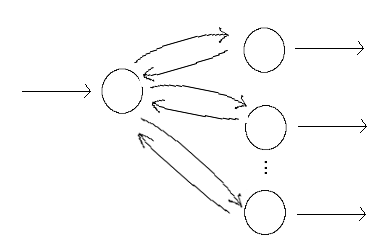
\includegraphics[scale=0.55]{map_no_g}
\caption{Structure of the implemented decomposition}
\label{fig:worker}
\end{figure} 




\end{document}
